\subsection{Electromagnetic Induction and Eddy Currents}
When supplied with an AC-voltage $U_0$, a coil will create an oscillating magnetic field $B_L$. If arranged in a closed electric circuit, a phase difference between voltage $U_L$ and current $I$ will occur in the coil. The correlation between voltage and current is defined as the coil impedance $Z_L:=U_L/I=R_L+\text{j}X_L$, where $R_L$ characterizes the resistance of the coil and $X_L = \omega L$ its reactance. The reactance depends on the AC-frequency $\omega$ and the inductance of the coil. 
\par
When an electrically conductive material is present, the magnetic field created by the coil induces eddy currents $I_c$ in the material. These currents cause power dissipation in the material as well as creating a secondary magnetic field $B_m$ that opposes the primary field. Therefore, the impedance of the coil changes to $Z'=R_L'+\text{j}X_L'$: its resistance increases due to the power loss while the reactance decreases with decreasing strength of the overall magnetic field.
\par
If the investigated material is ferromagnetic, the effects described above still occur. However, the ferromagnetic material also increases the primary magnetic field, exceeding the effect of the secondary field\cite{eddyCurrent}. Hence, the reactance of the coil is increased instead of being lowered (see figure\ref{fig:CoilImpedance}).

\subsection{Crack Detection}
\begin{figure}[htbp]
	\centering
		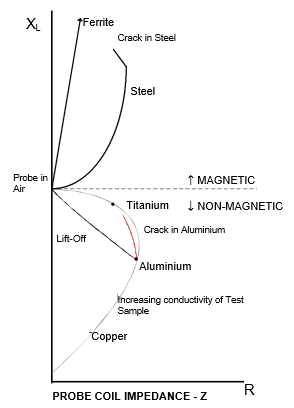
\includegraphics[width=0.3\textwidth]{img/CoilImpedance}
	\caption{the impedance $Z$ of the probe as a function of scanned material\cite{coilImpedance}}
	\label{fig:CoilImpedance}
\end{figure}
When cracks are present in the material (at the position of the probe), they impede the flow of eddy currents, thus decreasing the power dissipation and the strength of the secondary magnetic field. As a consequence, the coil's resistance changes to $R_L''$ (where $R_L<R_L''<R_L'$) and its reactance changes to $X_L''$ (where $X_L>X_L''>X_L'$ for non-ferromagnetic materials and $X_L''>X_L'>X_L$ for ferromagnetic materials respectively) as seen in figure\ref{fig:CoilImpedance}.

\subsection{Calculation of resistivity}
From electromagnetic theory we have that the induced current density $J$ at a given depth $d$ from an external field in a conductor is given by
\begin{equation}
\mathbf{J} = \mathbf{J_s} e^{-d/\delta}
\label{eq:th_Js}
\end{equation}
where $Js$ is the current density at surface of the metal and $\delta$
is the skin depth given by
\begin{equation}
\delta = \sqrt{\frac{2\rho}{\omega \mu}}
\label{eq:th_skindepth}
\end{equation}
where $\omega$ is the angular frequency of the current, $\mu$ is magnetic permeability and
$\rho$ is the resistivity.
Furthermore the electric field in a conductor is given by
\begin{equation}
\mathbf{E} = \rho \mathbf{J}.
\label{eq:th_E}
\end{equation}

Using eq. (\ref{eq:th_Js}), (\ref{eq:th_skindepth}) and (\ref{eq:th_E}) together with the equation for Joule heating we get
\begin{equation}
P_{loss}(d) = \mathbf{E}\cdot\mathbf{J} = \frac{1}{\rho}E^2.
\end{equation}
From eq. (\ref{eq:th_Js}) and (\ref{eq:th_E}) we have that $\mathbf{E} \propto e^{-d/\delta}$ and so
\begin{equation}
P_{loss}(d) \propto \frac{1}{\rho} e^{-2d/\delta},
\end{equation}
to get the total power loss $P_c$ we integrate over the thickness of the metal
\begin{equation}
P_{c} = \int_{0}^{D} P_{loss} (d) \approx \int_{0}^{\infty} P_{loss}(d) = \frac{C'}{\rho} \int_{0}^{\infty} e^{-2d/\delta} = \frac{C}{\rho} \delta
\end{equation}
where $C'$ and $C''$ are some constants; we can calculate the integral over infinite depth as long as the thickness $D$ of the metal is much larger than $\delta$.
Holding everything but $\rho$ fixed and using eq. \ref{eq:th_skindepth} we get that
\begin{equation}
P_{c} = C \sqrt{\rho}
\label{eq:P_metal}
\end{equation}
where $C$ is some constant.

This power loss due to heating in the conductor equivalently mean increased resistance in the source of the external field, from Ohm's law
\begin{equation}
P_{ohm} = \Re(\Delta U_L) I
\end{equation}
where $\Delta U_L$ is the change in the real part of the voltage and $I$ is the current of the external field source which is defined as without phase. Since $P_{ohm} = P_{c}$ we finally get that
\begin{equation}
\Re(\Delta U_L) I = C \sqrt{\rho}.
\label{eq:resistivity}
\end{equation}
assume $I_s$ is constant and this simplifies to
\begin{equation}
\rho = \left(\frac{\Re(\Delta U_L)}{C}\right)^2
\label{eq:resistivity_simp}
\end{equation}
for some other constant $C$.